\documentclass[12pt,a4paper]{article}

\usepackage{fontspec}
\usepackage{polyglossia}
\setmainlanguage{vietnamese}
\setotherlanguage{english}
\setmainfont{DejaVu Serif}
\setsansfont{DejaVu Sans}
\setmonofont{DejaVu Sans Mono}
\usepackage[margin=2.3cm]{geometry}
\usepackage{amsmath,amssymb}
\usepackage{graphicx}
\usepackage{listings}
\usepackage{xcolor}
\usepackage{booktabs}
\usepackage{tabularx}
\usepackage{enumitem}
\emergencystretch=3em
\usepackage{hyperref}
\usepackage{titlesec}
\usepackage{fancyhdr}

\hypersetup{colorlinks=true, linkcolor=blue!50!black, urlcolor=blue!50!black, citecolor=blue!50!black}

\titleformat{\section}{\normalfont\Large\bfseries}{\thesection}{1em}{}
\titleformat{\subsection}{\normalfont\large\bfseries}{\thesubsection}{1em}{}

\setlength{\headheight}{14pt}
\pagestyle{fancy}
\fancyhf{}
\rhead{CO2036}
\lhead{Xử lý tín hiệu số}
\cfoot{\thepage}

\definecolor{codebg}{RGB}{245,245,245}
\lstdefinelanguage{Scilab}{
  morekeywords={function,endfunction,if,then,else,elseif,end,for,while,do,break,return},
  sensitive=true,
  morecomment=[l]{//},
  morestring=[b]"
}
\lstset{
  backgroundcolor=\color{codebg},
  basicstyle=\ttfamily\small,
  language=Scilab,
  keywordstyle=\color{blue!60!black}\bfseries,
  commentstyle=\color{green!45!black},
  stringstyle=\color{orange!70!black},
  showstringspaces=false,
  breaklines=true,
  frame=single,
  rulecolor=\color{gray!50},
  numbers=left,
  numberstyle=\tiny\color{gray},
  xleftmargin=1.5em,
}

\newcommand{\solved}{\vspace{2mm}\noindent\textbf{Lời giải.}}

\begin{document}

%=====================================================================
% TRANG BÌA
%=====================================================================
\begin{titlepage}
\centering
\vspace*{1cm}
\vspace{1.5cm}
{\Huge\bfseries BÀI THỰC HÀNH XỬ LÝ TÍN HIỆU SỐ\par}
\vspace{0.5cm}
\vspace{2.5cm}
{\large Phạm Huỳnh Trọng Trí -- 2213657\par}
\vfill
{\large 27/09/2026\par}
\end{titlepage}

\tableofcontents
\newpage

%=====================================================================
\section*{Tổng Quan}
\addcontentsline{toc}{section}{Tổng Quan}
%=====================================================================

Làm quen với phần mềm SciLab, thực hiện các
thao tác vector cơ bản và minh họa quá trình lấy mẫu (sampling), lượng tử hóa
(quantization) một tín hiệu tương tự; và ôn tập lý thuyết tín
hiệu và hệ thống rời rạc theo thời gian (tín hiệu cơ bản, tính chẵn/lẻ, các phép
biến đổi tín hiệu) kết hợp thực hành dựng và thao tác các tín hiệu này trên SciLab.

%=====================================================================
\section{Giới Thiệu}
%=====================================================================

Lab 1 bài thực hành đầu tiên nhằm làm quen với công cụ SciLab -- phần mềm tính
toán số mã nguồn mở -- và áp dụng nó để minh họa hai bước rời rạc hóa nói trên.
Lab 2 tập trung vào nền tảng lý thuyết tín hiệu và hệ thống rời
rạc theo thời gian (discrete-time signal and system) đã học ở phần lý thuyết Với mỗi bài tập của cả hai lab, báo cáo trình bày đoạn
mã nguồn, hình vẽ minh họa và phần giải thích kết quả quan sát được.

%=====================================================================
\section{Mục Tiêu}
%=====================================================================

Sau khi hoàn thành hai bài thực hành, đạt được các mục tiêu sau:

\begin{itemize}[leftmargin=1.2em]
  \item Làm quen với môi trường SciLab: console, editor (SciNotes), cửa sổ đồ thị.
  \item Thực hiện được các phép toán cơ bản trên vector (cộng, nhân từng phần tử,
  áp dụng hàm lượng giác) bằng các lệnh \texttt{:}, \texttt{linspace}, và các toán
  tử \texttt{+}, \texttt{.*}.
  \item Ôn tập lý thuyết về tín hiệu và hệ thống rời rạc theo thời gian: tín hiệu
  cơ bản, tính chẵn/lẻ, năng lượng và công suất tín hiệu, các phép biến đổi tín
  hiệu.
  \item Nắm được cách sử dụng các hàm SciLab thường dùng khi xử lý tín hiệu rời
  rạc: \texttt{plot2d3}, \texttt{bool2s}, \texttt{subplot}, \texttt{title},
  \texttt{xlabel}, \texttt{ylabel}, \texttt{min}, \texttt{max}, \texttt{deff}.
\end{itemize}

%=====================================================================
\section{Phương Pháp}
%=====================================================================

\textbf{Phần mềm sử dụng.} SciLab có các hàm, công cụ tính toán
số được dùng xuyên suốt cả hai bài thực hành.

%=====================================================================
\section{Nội Dung Thực Hành}
%=====================================================================

\subsection{Bài 1 -- Lab 1: Vector Cơ Bản, Lấy Mẫu và Lượng Tử Hóa}

\subsubsection*{1.1 Thao tác vector}

Sử dụng vector $x = 1{:}4$ và $y = 5{:}8$, thực hiện các phép toán sau:

\begin{lstlisting}[caption=Ex 1.1 -- Thao tác vector]
// (a) cong 1 vao moi phan tu
x = 1:4;
y1 = x + 1

// (b) nhan tung phan tu
x = 1:4;
y = 5:8;
y2 = x .* y

// (c) sin cua 10 diem chia deu trong [0, pi]
x = linspace(0, %pi, 10);
y3 = sin(x)
\end{lstlisting}

\textbf{Nhận xét:} phép cộng và phép nhân với một hằng số áp dụng mặc định theo
kiểu từng phần tử (element-wise). Tuy nhiên với hai vector cùng kích thước, phải
dùng toán tử \texttt{.*} (không phải \texttt{*}) để nhân tương ứng từng phần tử,
vì \texttt{*} được SciLab hiểu là phép nhân ma trận.
\begin{center}
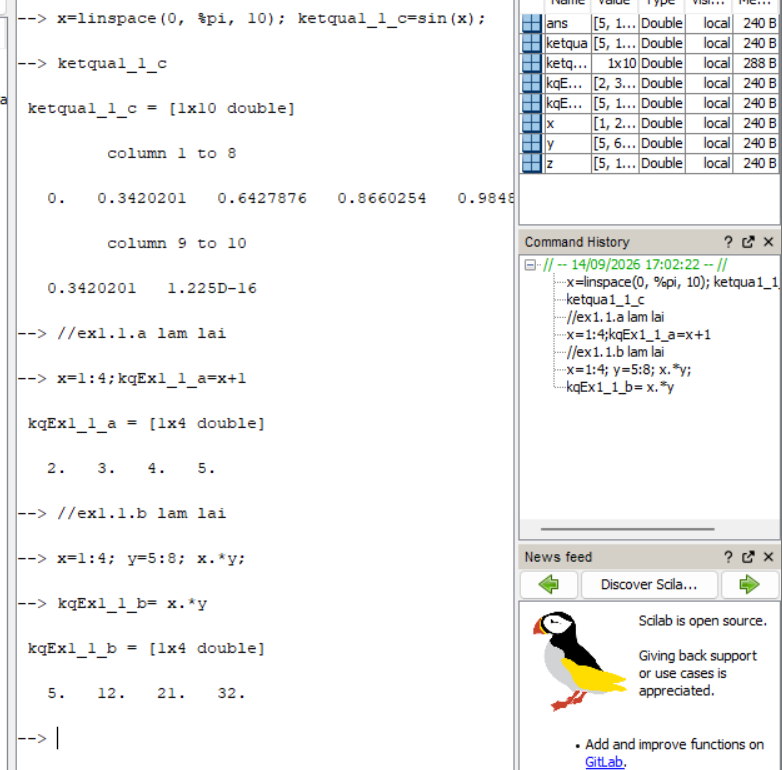
\includegraphics[width=0.62\textwidth]{lab1_ex1.png}
\textit{ on-screen scene scilab }
\end{center}

\subsubsection*{1.2 Lấy mẫu và lượng tử hóa tín hiệu}

Cho tín hiệu tương tự $x_a(t) = 3\sin(100\pi t)$.

\textbf{(a) Vẽ $x_a(t)$ trong 5 chu kỳ.} Từ $\Omega = 100\pi$ suy ra $f = 50$~Hz,
chu kỳ $T_a = 0{,}02$~s, nên 5 chu kỳ tương ứng khoảng thời gian $0{,}1$~s.

\textbf{(b) Xác định $x(n)$ khi lấy mẫu với $F_s = 300$ mẫu/giây.} Thay
$t = n/F_s$ vào $x_a(t)$:
\[
x(n) = 3\sin\!\left(100\pi \cdot \frac{n}{300}\right) = 3\sin\!\left(\frac{\pi}{3}n\right)
\]

\textbf{(c) Tính tuần hoàn.} Với $\omega_0 = \pi/3$:
\[
\frac{\omega_0}{2\pi} = \frac{1}{6}
\]
là số hữu tỉ dạng $k/N$ với $k=1$, $N=6$ $\Rightarrow$ $x(n)$ tuần hoàn với chu kỳ
$N = 6$ mẫu; 5 chu kỳ tương ứng $30$ mẫu.

\textbf{(d) Lượng tử hóa} với $\Delta = 0{,}1$, phương pháp truncation:
\[
x_q(n) = \Delta \cdot \left\lfloor \frac{x(n)}{\Delta} \right\rfloor
\]

\begin{lstlisting}[caption=Ex 1.2 -- Lay mau va luong tu hoa]
// (a) tin hieu tuong tu
t = linspace(0, 0.1, 1000);
xa = 3*sin(100*%pi*t);
subplot(3,1,1)
plot(t, xa)
xtitle("x_a(t) = 3sin(100*pi*t)")

// (b),(c) tin hieu lay mau, Fs=300Hz, chu ky N=6 mau
n = 0:29;
xn = 3*sin(%pi/3*n);
subplot(3,1,2)
plot2d3(n, xn)
xtitle("x(n), N=6 mau/chu ky (5 chu ky = 30 mau)")

// (d) luong tu hoa, Delta=0.1, truncation
delta = 0.1;
xq = delta * floor(xn/delta);
subplot(3,1,3)
plot2d3(n, xq)
xtitle("x_q(n), Delta=0.1 (truncation)")
\end{lstlisting}

\begin{center}
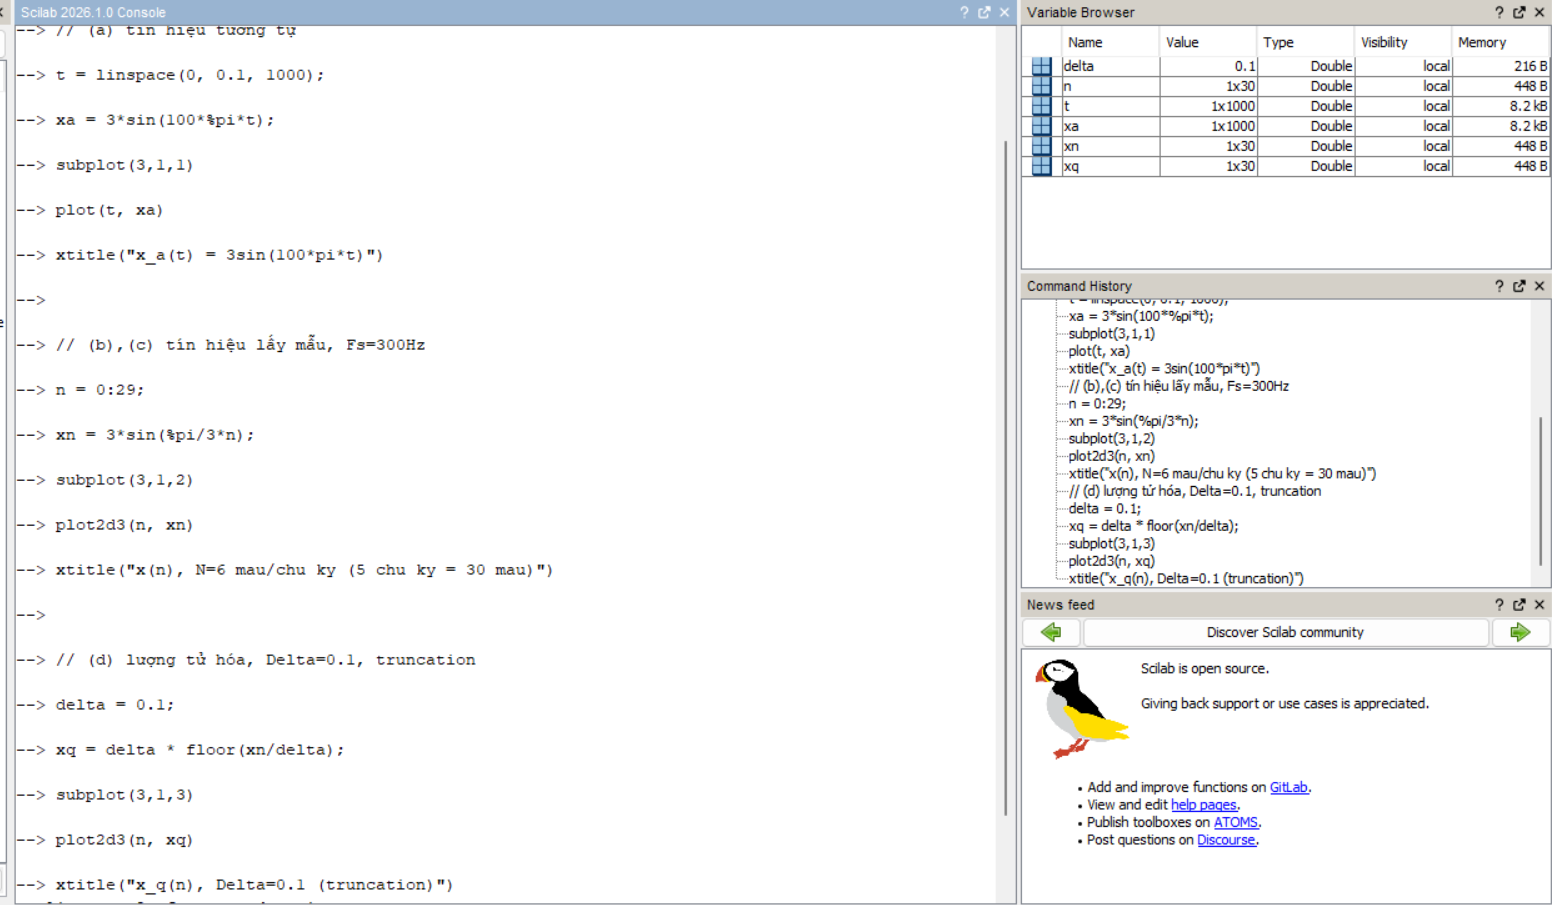
\includegraphics[width=0.62\textwidth]{lab1_ex2.png}
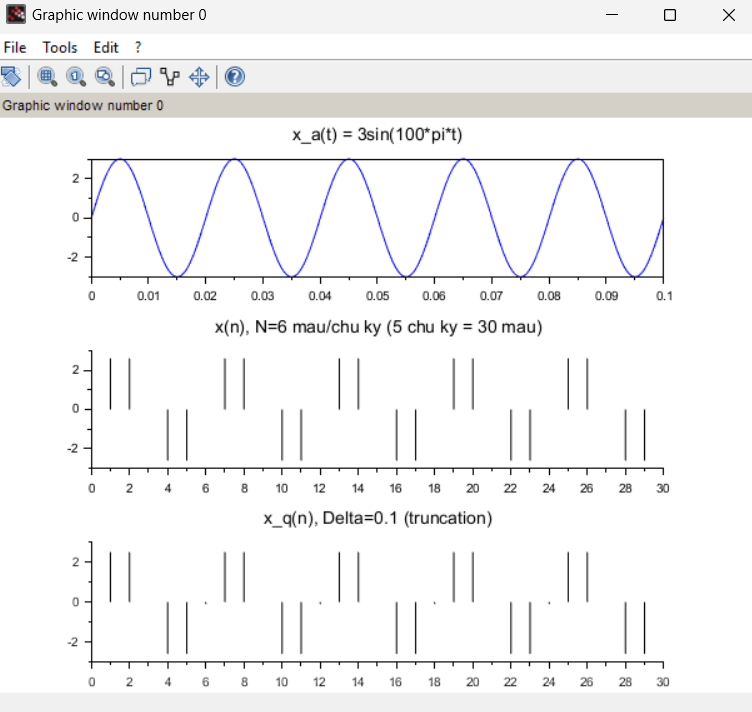
\includegraphics[width=0.62\textwidth]{lab1_ex2_result.png}
\textit{ on-screen scene scilab }
\end{center}

\textbf{Nhận xét chung Bài 1:} đã minh họa được toàn bộ chuỗi xử lý tín hiệu: từ
tín hiệu tương tự liên tục, qua bước lấy mẫu để thành tín hiệu rời rạc theo thời
gian, rồi qua bước lượng tử hóa để thành tín hiệu số hoàn chỉnh.

\subsection{Bài 2 -- Lab 2: Tín Hiệu và Hệ Thống Rời Rạc Theo Thời Gian}

\subsubsection{Ôn tập lý thuyết}
\label{sec:review}

\paragraph{Tín hiệu cơ bản}

\begin{itemize}[leftmargin=1.2em]
  \item \textbf{Xung đơn vị (unit sample sequence)}
  \[
    \delta(n) = \begin{cases} 1, & n = 0 \\ 0, & n \neq 0 \end{cases}
  \]
  \item \textbf{Tín hiệu bước đơn vị (unit step)}
  \[
    u(n) = \begin{cases} 1, & n \geq 0 \\ 0, & n < 0 \end{cases}
  \]
  \item \textbf{Tín hiệu dốc đơn vị (unit ramp)}
  \[
    u_r(n) = \begin{cases} n, & n \geq 0 \\ 0, & n < 0 \end{cases}
  \]
\end{itemize}

\paragraph{Tính chất của tín hiệu}

\begin{itemize}[leftmargin=1.2em]
  \item \textbf{Tín hiệu tuần hoàn.} $x(n)$ tuần hoàn với chu kỳ $N$ $(N>0)$ khi và
  chỉ khi $x(n+N) = x(n),\ \forall n$.

  \item \textbf{Năng lượng tín hiệu}
  \[
    E_x = \sum_{n=-\infty}^{\infty} |x(n)|^2 .
  \]

  \item \textbf{Công suất trung bình}
  \[
    P_x = \lim_{N\to\infty}\frac{1}{2N+1}\sum_{n=-N}^{N} |x(n)|^2 .
  \]

  \item \textbf{Tính đối xứng (chẵn/lẻ).} Mọi tín hiệu bất kỳ có thể phân tích
  thành tổng của thành phần chẵn và thành phần lẻ:
  \[
    x(n) = x_e(n) + x_o(n),
  \]
  \[
    x_e(n) = \tfrac{1}{2}\big[x(n)+x(-n)\big] \ \text{(chẵn)}, \qquad
    x_o(n) = \tfrac{1}{2}\big[x(n)-x(-n)\big] \ \text{(lẻ)}.
  \]
\end{itemize}

\paragraph{Các phép biến đổi tín hiệu cơ bản}

\begin{itemize}[leftmargin=1.2em]
  \item \textbf{Dịch trễ (delay):} $y(n) = x(n-k)$, \ $k>0$
  \item \textbf{Dịch sớm (advance):} $y(n) = x(n+k)$, \ $k>0$
  \item \textbf{Gấp (folding):} $y(n) = x(-n)$
  \item \textbf{Cộng (addition):} $y(n) = x_1(n) + x_2(n)$
  \item \textbf{Nhân (multiplication):} $y(n) = x_1(n)\cdot x_2(n)$
  \item \textbf{Tỷ lệ biên độ (amplitude scaling):} $y(n) = a\,x(n)$
\end{itemize}

\subsubsection{Khảo sát các hàm SciLab}

\begin{center}
\begin{tabularx}{\textwidth}{@{}lX@{}}
\toprule
\textbf{Hàm} & \textbf{Chức năng} \\
\midrule
\texttt{plot2d3(x,y)} & Vẽ dữ liệu rời rạc dạng các vạch đứng (kiểu ``stem'') từ trục
  hoành lên tới giá trị $y(n)$ -- cách chuẩn để hiển thị tín hiệu rời rạc theo thời
  gian trong SciLab.\\[2pt]
\texttt{min(x)} & Trả về phần tử nhỏ nhất của vector/ma trận \texttt{x} (có thể kèm
  chỉ số của phần tử nhỏ nhất). \\[2pt]
\texttt{max(x)} & Trả về phần tử lớn nhất của vector/ma trận \texttt{x} (có thể kèm
  chỉ số của phần tử lớn nhất). \\[2pt]
\texttt{subplot(m,n,k)} & Chia cửa sổ đồ thị hiện tại thành lưới $m\times n$ ô, và
  chọn ô thứ $k$ làm ô hiện hành cho lệnh vẽ tiếp theo. \\[2pt]
\texttt{title("...")} & Đặt tiêu đề hiển thị phía trên trục tọa độ hiện hành. \\[2pt]
\texttt{xlabel("...")} & Đặt nhãn cho trục hoành của trục tọa độ hiện hành. \\[2pt]
\texttt{ylabel("...")} & Đặt nhãn cho trục tung của trục tọa độ hiện hành. \\[2pt]
\texttt{bool2s(cond)} & Chuyển một mảng boolean (kết quả của phép so sánh logic như
  \texttt{n>=0}) thành mảng số 0/1 -- rất tiện để tạo các tín hiệu dạng bước từ điều
  kiện logic. \\[2pt]
\texttt{deff("[y]=f(x)","y=...")} & Định nghĩa nhanh một hàm SciLab \texttt{f} từ hai
  chuỗi (phần khai báo và phần thân hàm) mà không cần tạo file \texttt{.sci} riêng. \\
\bottomrule
\end{tabularx}
\end{center}

\paragraph{Bài tập 2 -- Tín hiệu bước đơn vị qua \texttt{bool2s}}

\begin{lstlisting}
n = -5:5;
msignal = bool2s(n >= 0);
plot2d3(n, msignal)
xlabel('n'); ylabel('u(n)');
title('Unit step u(n)');
\end{lstlisting}

\solved Phép so sánh \texttt{n>=0} tạo ra vector boolean bằng \texttt{\%T} với
$n\ge0$ và \texttt{\%F} với $n<0$; \texttt{bool2s} chuyển vector này thành vector số
$\{0,0,0,0,0,1,1,1,1,1,1\}$ ứng với $n=-5,\dots,5$ -- chính là tín hiệu bước đơn vị
$u(n)$ giới hạn trong cửa sổ $[-5,5]$.
\begin{center}
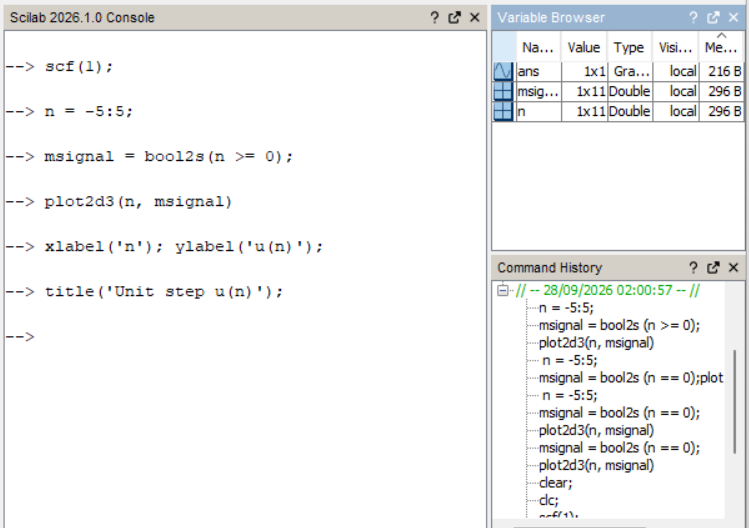
\includegraphics[width=0.62\textwidth]{lab2_ex2.png}
\textit{ on-screen scene scilab }
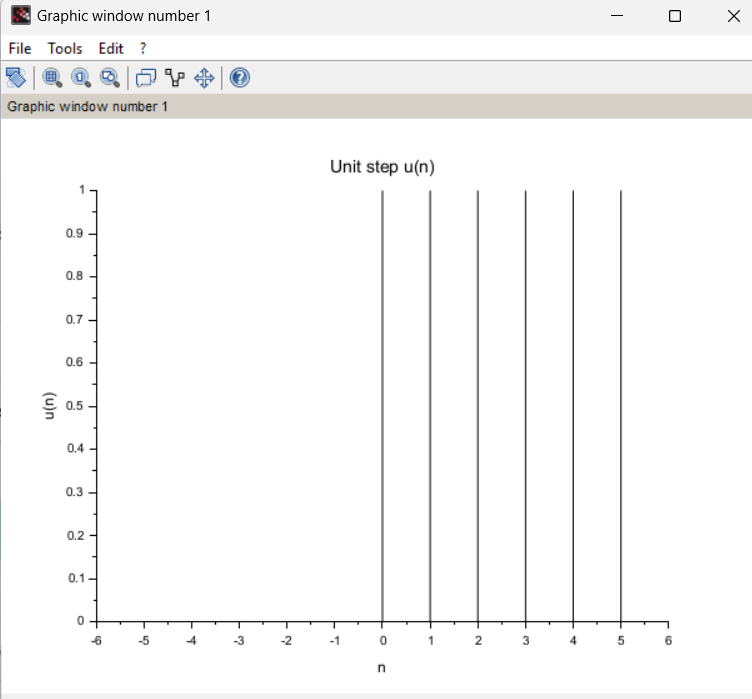
\includegraphics[width=0.62\textwidth]{lab2_ex2_graphic.png}
\end{center}

\begin{center}
\textit{(Hình: đồ thị $u(n)$)}
\end{center}

\paragraph{Bài tập 3 -- Xung đơn vị qua \texttt{bool2s}}

\begin{lstlisting}
n = -5:5;
msignal = bool2s(n == 0);
plot2d3(n, msignal)
xlabel('n'); ylabel('delta(n)');
title('Unit impulse delta(n)');
\end{lstlisting}

\solved Điều kiện \texttt{n==0} chỉ đúng tại chỉ số $n=0$, nên \texttt{msignal} là
vector $\{0,\dots,0,1,0,\dots,0\}$ với giá trị 1 duy nhất tại $n=0$ -- chính là xung
đơn vị $\delta(n)$.

\begin{center}
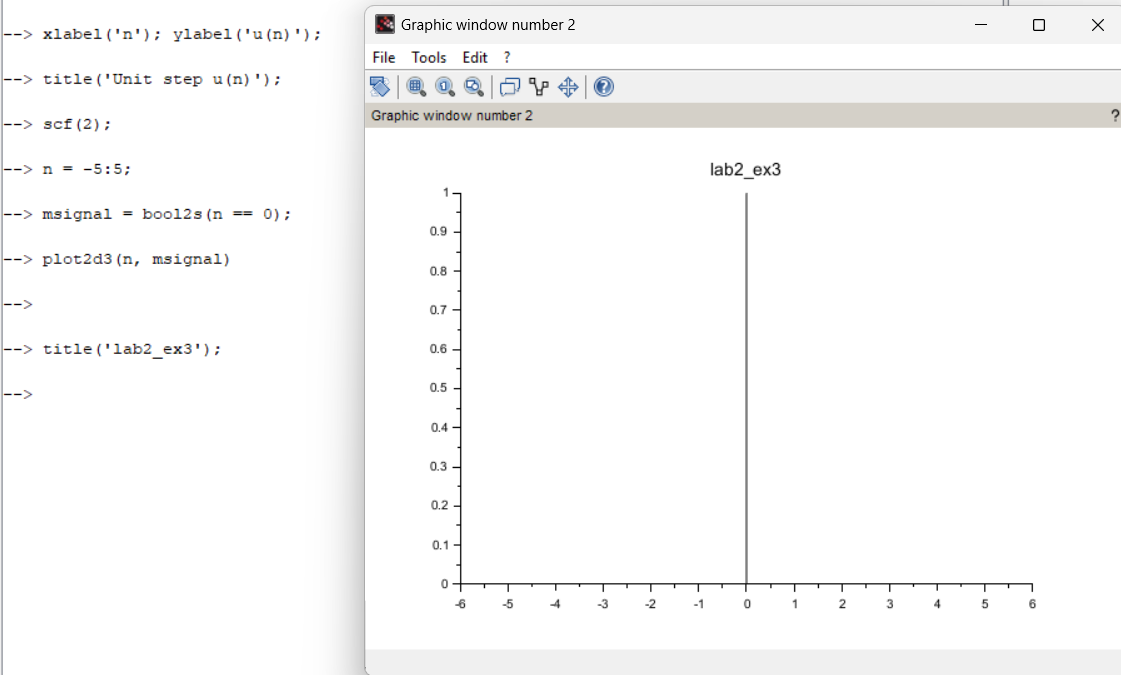
\includegraphics[width=0.62\textwidth]{lab2_ex3_graphic.png}
\end{center}

\begin{center}
\textit{(Hình: đồ thị $\delta(n)$)}
\end{center}

\paragraph{Bài tập 4 -- Tín hiệu dốc đơn vị $u_r(n)$, $n=-5\!:\!5$}

\begin{lstlisting}
n = -5:5;
ur = n .* bool2s(n >= 0);   // ur(n) = n voi n>=0, 0 nguoc lai
plot2d3(n, ur)
xlabel('n'); ylabel('ur(n)');
title('Unit ramp ur(n)');
\end{lstlisting}

\solved Phép nhân từng phần tử \texttt{n .* bool2s(n>=0)} giữ nguyên giá trị $n$ khi
$n\ge 0$ và triệt tiêu khi $n<0$, cho ra
$u_r(n) = \{0,0,0,0,0,0,1,2,3,4,5\}$ với $n=-5,\dots,5$.

\begin{center}
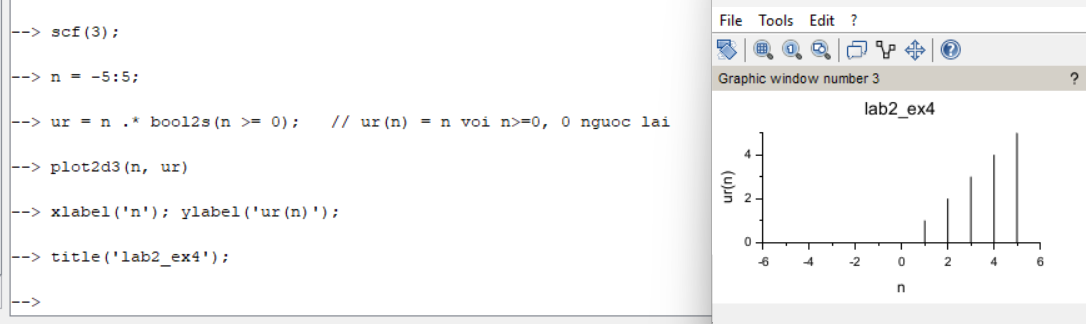
\includegraphics[width=0.62\textwidth]{lab2_ex4_graphic.png}
\end{center}

\begin{center}
\textit{(Hình: đồ thị $u_r(n)$)}
\end{center}

\paragraph{Bài tập 5 -- Phân tích chẵn/lẻ của $x(n)=\{1,\underset{\uparrow}{3},-2\}$}

Mũi tên đánh dấu $n=0$, nên $x(-1)=1,\ x(0)=3,\ x(1)=-2$.

\solved Áp dụng $x_e(n)=\tfrac12[x(n)+x(-n)]$ và $x_o(n)=\tfrac12[x(n)-x(-n)]$ trên
miền $n\in\{-1,0,1\}$:
\[
x(-n):\ \{-2,3,1\}, \qquad
x_e(n) = \{-0.5,\,3,\,-0.5\}, \qquad
x_o(n) = \{1.5,\,0,\,-1.5\}.
\]
Kiểm tra: $x_e(n)+x_o(n) = \{1,3,-2\} = x(n)$. \checkmark

\begin{lstlisting}
n  = -1:1;
x  = [1 3 -2];
xr = x($:-1:1);          // x(-n) tren cung mien (lat vector)
xe = 0.5*(x + xr);       // thanh phan chan
xo = 0.5*(x - xr);       // thanh phan le

subplot(3,1,1); plot2d3(n,x);  title('x(n)');  xlabel('n'); ylabel('x(n)');
subplot(3,1,2); plot2d3(n,xe); title('xe(n)'); xlabel('n'); ylabel('xe(n)');
subplot(3,1,3); plot2d3(n,xo); title('xo(n)'); xlabel('n'); ylabel('xo(n)');
\end{lstlisting}

\begin{center}
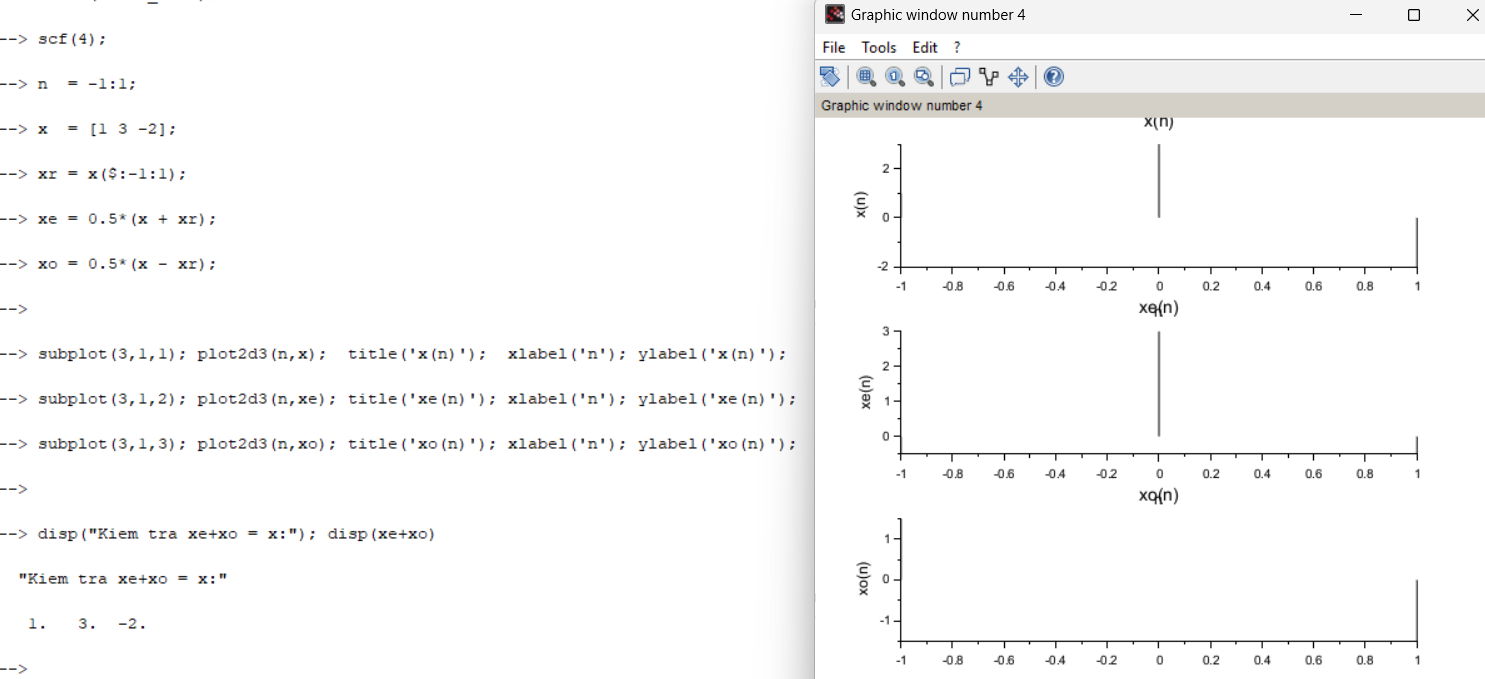
\includegraphics[width=0.62\textwidth]{lab2_ex5_graphic.png}
\end{center}

\begin{center}
\textit{(Hình: $x(n)$, $x_e(n)$, $x_o(n)$)}
\end{center}

\paragraph{Bài tập 6 -- Phép cộng: $y(n)=x_1(n)+x_2(n)$}

$x_1(n)=\{\underset{\uparrow}{0},1,3,-2\}$ (miền $n=0,1,2,3$), \quad
$x_2(n)=\{0,\underset{\uparrow}{1},2,3\}$ (miền $n=-1,0,1,2$).

\solved Đệm 0 cho mỗi tín hiệu ngoài miền xác định của nó rồi gộp trên miền chung
$n=-1,\dots,3$:

\begin{center}
\begin{tabular}{c|ccccc}
$n$      & $-1$ & $0$ & $1$ & $2$ & $3$ \\ \hline
$x_1(n)$ & $0$  & $0$ & $1$ & $3$ & $-2$ \\
$x_2(n)$ & $0$  & $1$ & $2$ & $3$ & $0$ \\ \hline
$y(n)$   & $0$  & $1$ & $3$ & $6$ & $-2$
\end{tabular}
\end{center}

\begin{lstlisting}
n1 = 0:3;        x1 = [0 1 3 -2];
n2 = -1:2;       x2 = [0 1 2 3];

n  = min(n1(1),n2(1)):max(n1($),n2($));  // mien chung, -1:3
y1 = zeros(1,length(n)); y2 = zeros(1,length(n));
y1(n1 - n(1) + 1) = x1;                  // dem 0 x1 tren truc chung
y2(n2 - n(1) + 1) = x2;                  // dem 0 x2 tren truc chung
y  = y1 + y2;

subplot(3,1,1); plot2d3(n,y1); title('x1(n)'); xlabel('n');
subplot(3,1,2); plot2d3(n,y2); title('x2(n)'); xlabel('n');
subplot(3,1,3); plot2d3(n,y);  title('y(n)=x1(n)+x2(n)'); xlabel('n');
\end{lstlisting}

\begin{center}
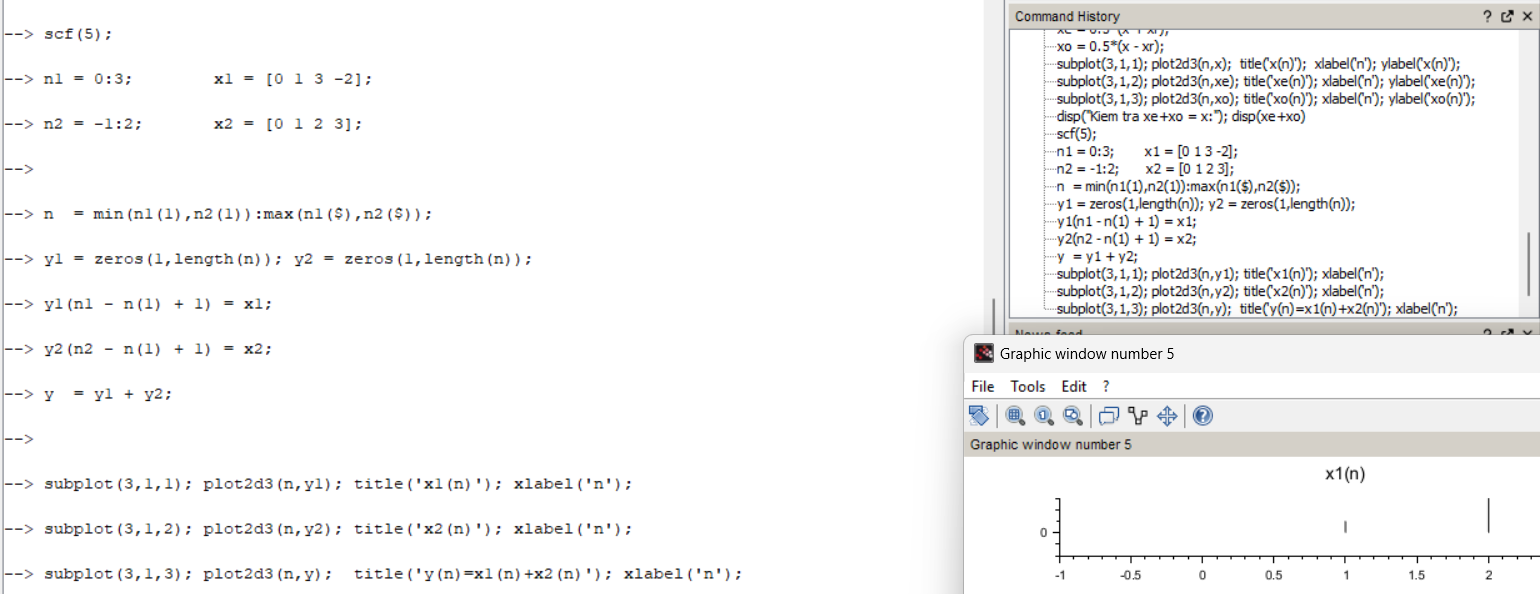
\includegraphics[width=0.62\textwidth]{lab2_ex6.png}
\textit{ on-screen scene scilab }
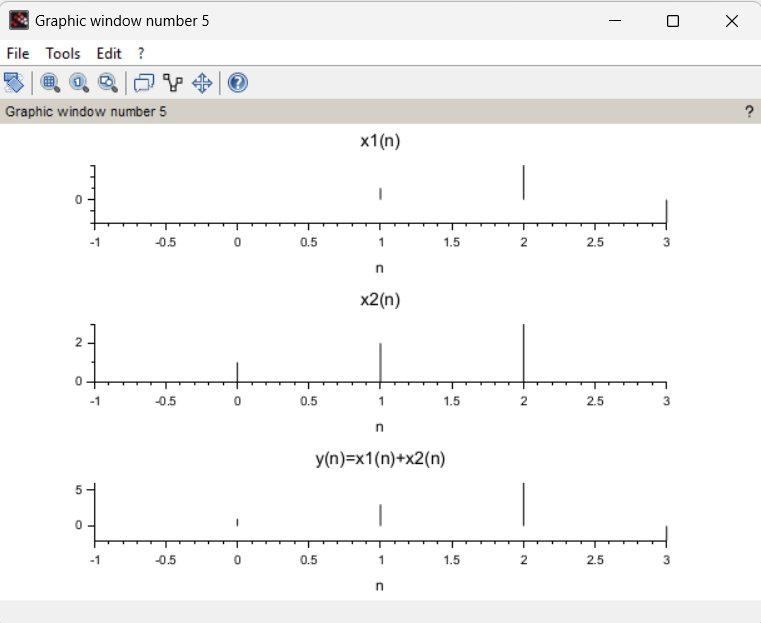
\includegraphics[width=0.62\textwidth]{lab2_ex6_graphic.png}
\end{center}

\begin{center}
\textit{(Hình: $x_1(n)$, $x_2(n)$, $y(n)=x_1(n)+x_2(n)$)}
\end{center}

\paragraph{Bài tập 7 -- Phép nhân: $y(n)=x_1(n)\cdot x_2(n)$}

Sử dụng lại $x_1(n),x_2(n)$ như Bài tập 6, gộp trên miền $n=-1,\dots,3$:

\begin{center}
\begin{tabular}{c|ccccc}
$n$      & $-1$ & $0$ & $1$ & $2$ & $3$ \\ \hline
$x_1(n)$ & $0$  & $0$ & $1$ & $3$ & $-2$ \\
$x_2(n)$ & $0$  & $1$ & $2$ & $3$ & $0$ \\ \hline
$y(n)$   & $0$  & $0$ & $2$ & $9$ & $0$
\end{tabular}
\end{center}

\begin{lstlisting}
// n, y1, y2 giong nhu Bai tap 6
y = y1 .* y2;             // nhan tung phan tu

subplot(3,1,1); plot2d3(n,y1); title('x1(n)'); xlabel('n');
subplot(3,1,2); plot2d3(n,y2); title('x2(n)'); xlabel('n');
subplot(3,1,3); plot2d3(n,y);  title('y(n)=x1(n).x2(n)'); xlabel('n');
\end{lstlisting}

\begin{center}
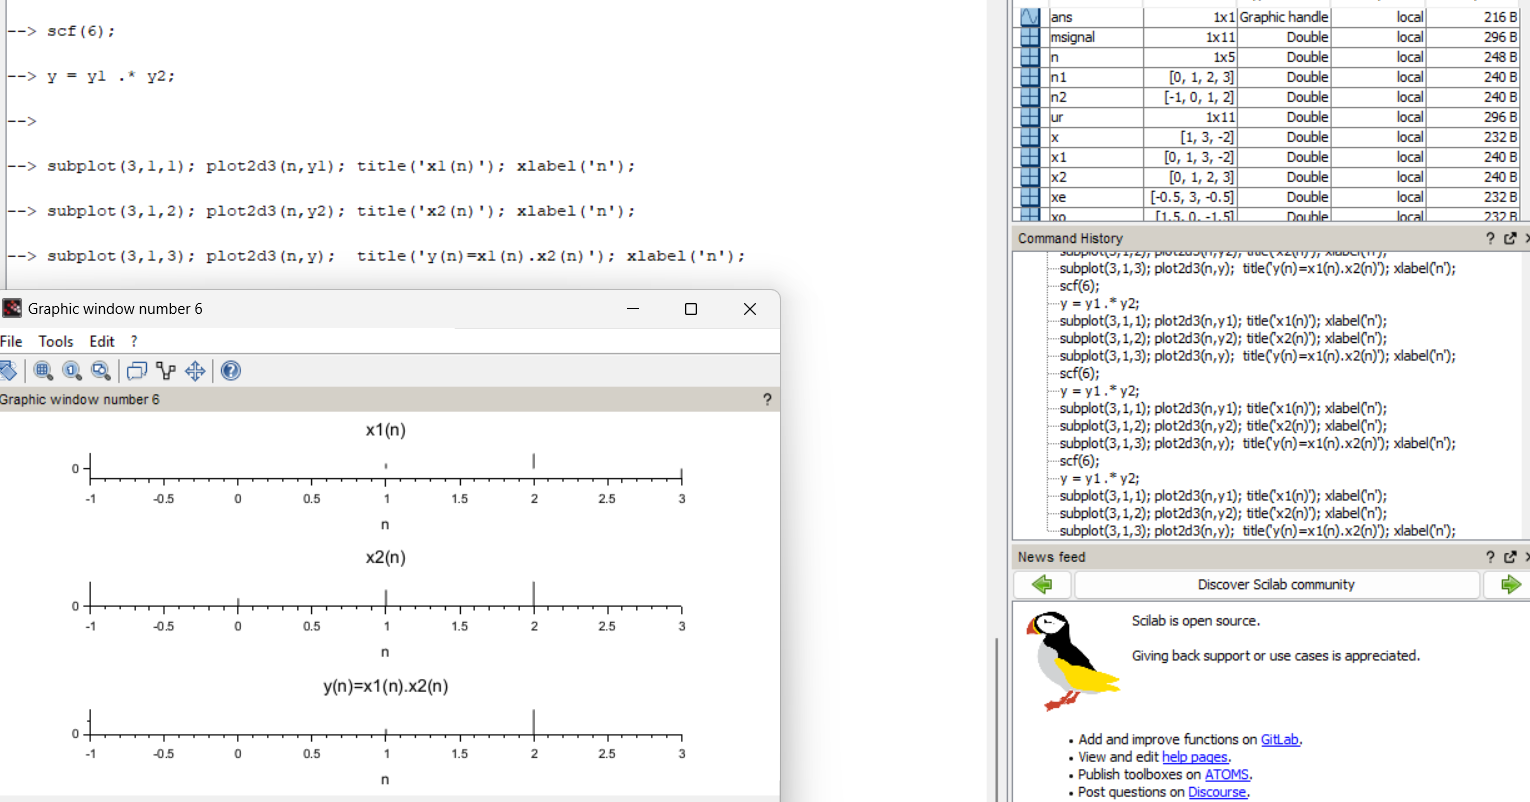
\includegraphics[width=0.62\textwidth]{lap2_ex7_graphic.png}
\end{center}

\begin{center}
\textit{(Hình: $x_1(n)$, $x_2(n)$, $y(n)=x_1(n)\cdot x_2(n)$)}
\end{center}

\paragraph{Bài tập 8 -- Gấp, dịch sớm và gấp-dịch có tỷ lệ}

$x(n) = \{1,-2,\underset{\uparrow}{3},6\}$, nên $x(-2)=1,\ x(-1)=-2,\ x(0)=3,\ x(1)=6$.

\solved
\[
y_1(n) = x(-n): \quad n=-1,0,1,2 \ \Rightarrow\ y_1 = \{6,3,-2,1\}
\]
\[
y_2(n) = x(n+3): \quad n=-5,-4,-3,-2 \ \Rightarrow\ y_2 = \{1,-2,3,6\}
\]
\[
y_3(n) = 2\,x(-n-2): \quad n=-3,-2,-1,0 \ \Rightarrow\ y_3 = \{12,6,-4,2\}
\]

\begin{lstlisting}
nx = -2:1;         x = [1 -2 3 6];

// y1(n) = x(-n)
n1 = -1:2;         y1 = x($:-1:1);

// y2(n) = x(n+3)  (dich som 3)
n2 = -5:-2;        y2 = x;

// y3(n) = 2*x(-n-2)
n3 = -3:0;         y3 = 2*x($:-1:1);

subplot(2,2,1); plot2d3(nx,x);  title('x(n)');
subplot(2,2,2); plot2d3(n1,y1); title('y1(n)=x(-n)');
subplot(2,2,3); plot2d3(n2,y2); title('y2(n)=x(n+3)');
subplot(2,2,4); plot2d3(n3,y3); title('y3(n)=2x(-n-2)');
\end{lstlisting}

\begin{center}
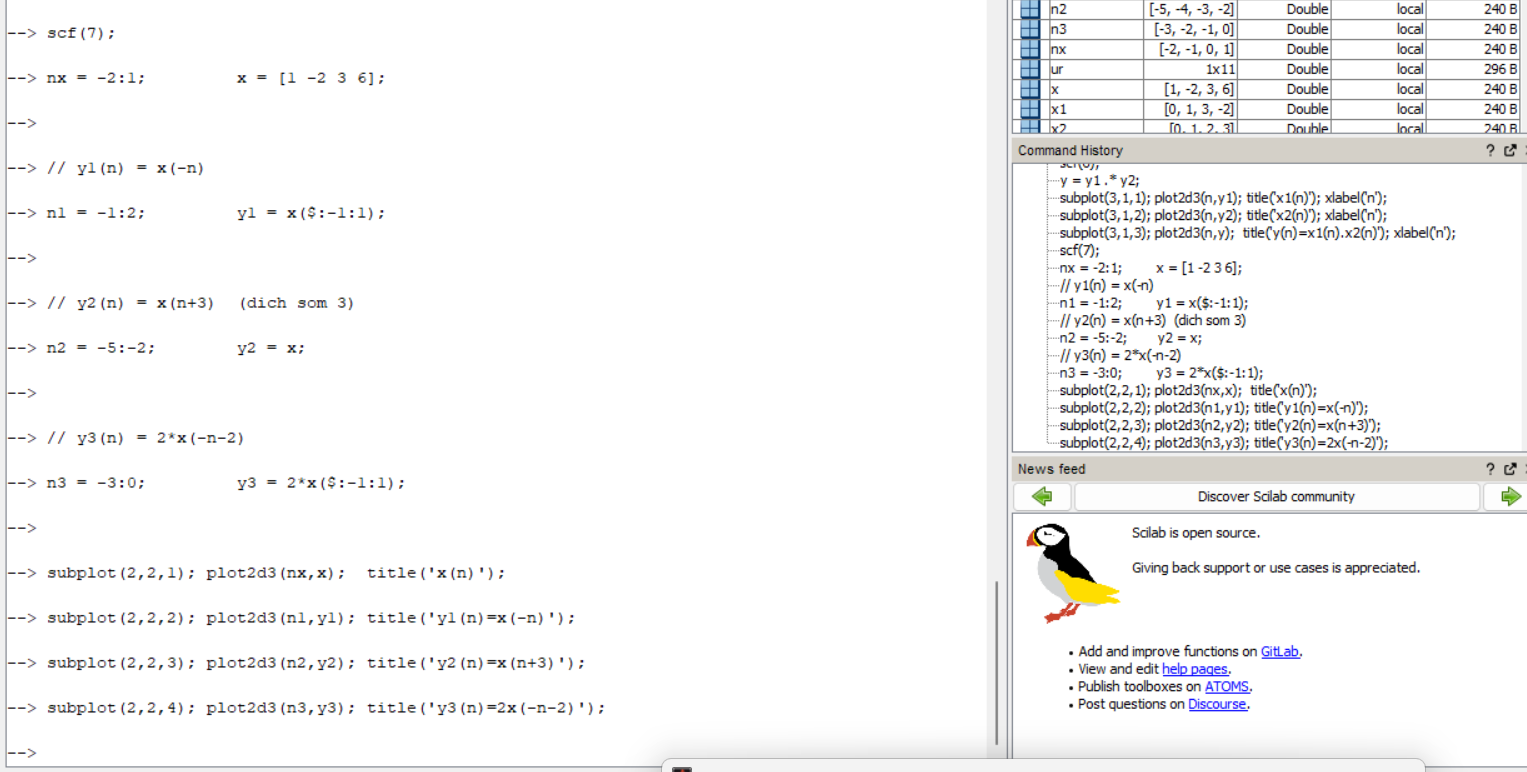
\includegraphics[width=0.62\textwidth]{lab2_ex8.png}
\textit{ on-screen scene scilab }
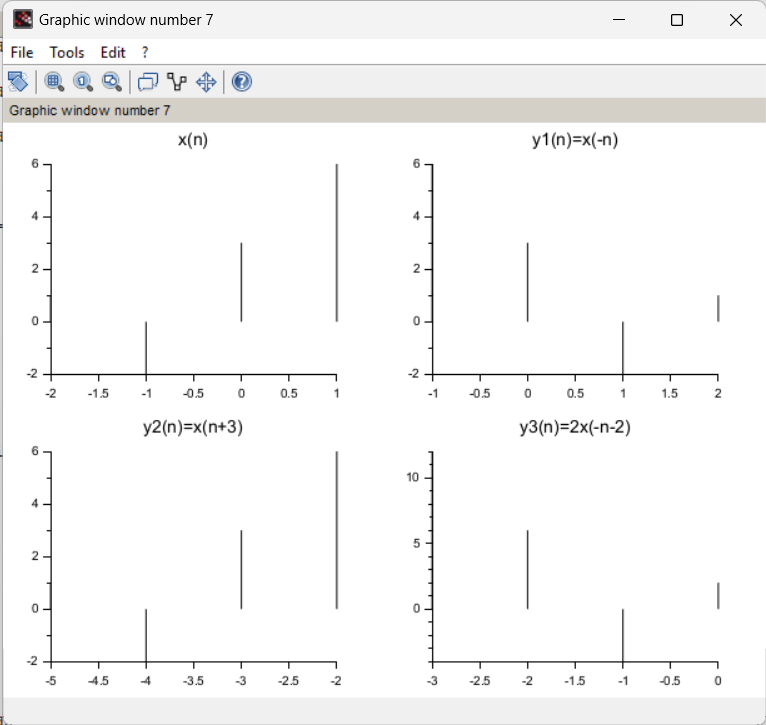
\includegraphics[width=0.62\textwidth]{lab2_ex8_graphic.png}
\end{center}

\begin{center}
\textit{(Hình: $x(n)$, $y_1(n)$, $y_2(n)$, $y_3(n)$)}
\end{center}

%=====================================================================
\section{Bàn Luận}
%=====================================================================

Qua hai bài thực hành, đã làm quen được với môi trường SciLab và thực hiện thành
công các thao tác vector cơ bản, minh họa toàn bộ chuỗi xử lý tín hiệu: từ tín hiệu
tương tự liên tục, qua bước lấy mẫu để thành tín hiệu rời rạc theo thời gian, rồi
qua bước lượng tử hóa để thành tín hiệu số hoàn chỉnh; đồng thời các khái
niệm lý thuyết về tín hiệu rời rạc (xung, bước, dốc đơn vị, tính chẵn/lẻ, các phép
biến đổi tín hiệu) cũng đã được minh họa cụ thể bằng SciLab, giúp liên kết chặt chẽ
giữa công thức toán học và cách biểu diễn tín hiệu trên máy tính.

Các điểm cần lưu ý: (1) sự khác biệt giữa toán tử \texttt{*} và \texttt{.*} trong
SciLab; (2) điều kiện để một tín hiệu rời rạc dạng sin là tuần hoàn (tỉ số
$\omega_0/2\pi$ phải là số hữu tỉ) -- một tính chất không có ở tín hiệu liên tục;

%=====================================================================
\section{Tài Liệu Tham Khảo}
%=====================================================================

\begin{enumerate}
  \item Mã nguồn SciLab của cả hai bài thực hành và báo cáo latex:
\url {https://github.com/nhd000/HK261_Report_L02_Lab_2213657}
\end{enumerate}

\end{document}
